\section{Experiments}
\label{experiments}
The modelling and experiments of this dissertation were split into two parts. The first part explored different topic modelling approaches, in an aim to build and use a curated topic model. This topic model was trained on event data filtered in GDELT where the events were only those concerning the USA or China. This topic model could then be used on more data from GDELT, to filter out new events where the headlines from the URLs which match the topics used in the topic model. The same GDELT filtered USA/China dataset was used to model the binary stock shift with the Goldstein Scale and Average Tone values. 

These two approaches were run concurrently, with the eventual aim being that they would be merged if the initial experiments were successful, and then tested on another dataset, to get a measure of how accurate and useful this method might be. 

\subsection{Data Acquisition}
There were 2 main sources of data acquisition, firstly data was taken from the GDELT Events table. This data was for the use of building the topic model, and getting the average tone and Goldstein scale values for the events on specific days. The second dataset to be used was data for the Dow Jones Industrial average which measures the stock performance of 30 large companies on stock exchanges across the United States, namely the NASDAQ and the New York Stock Exchange.

\subsubsection{GDELT}
The GDELT data was acquired using two different procedures, firstly a python package was used to retrieve the GDELT events table data for the single day of 1st of November 2019. Then using the Google Cloud platform, and Google Big Query, the larger USA China Dataset was taken. There were two main reasons for selecting this subset of data. Firstly, there was significant news being generated between the USA and China during this period, and the stock market remained volatile, thus it seemed most promising to find a relationship, and build a curated topic model. Secondly, the events table data had to be restricted, as there would be too much data to process on the machine the models were run on. 

After the data was collected, There was a significant chunk of processing required for the GDELT data. Firstly the URLs had to be parsed to get the headlines (where present, not all of the URLs had headlines which were usable). Then the words were stripped and made into a corpus of documents, to be used in the topic modelling. 

The Goldstein scale and average tone values were aggregated across the dates, and the results shown in Figures \ref{fig:avg_tone_diff} and \ref{fig:gs_diff}. Figure \ref{fig:avg_tone_diff} shows the daily Average tone of the events across days. This data is fairly chaotic, and thus the moving average for 3 days was plotted and is shown in Figure \ref{fig:avg_ma}. It is immediately apparent that the Average Tone is always negative, which is perhaps to be expected given the frosty relationship between the USA and China during the months of March and April. 
 
 \begin{figure}[H]
 	\centering
 	\subfloat[GDELT Average Tone]{  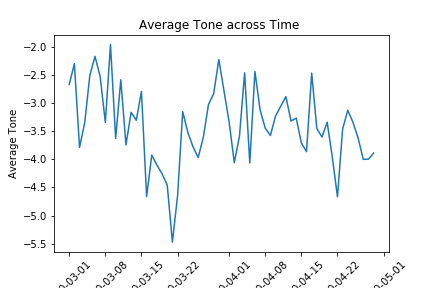
\includegraphics[width=0.49\textwidth]{images/avgtone.png}\label{fig:avg}}
 	\subfloat[GDELT Average Tone 3 Day Moving Average]{  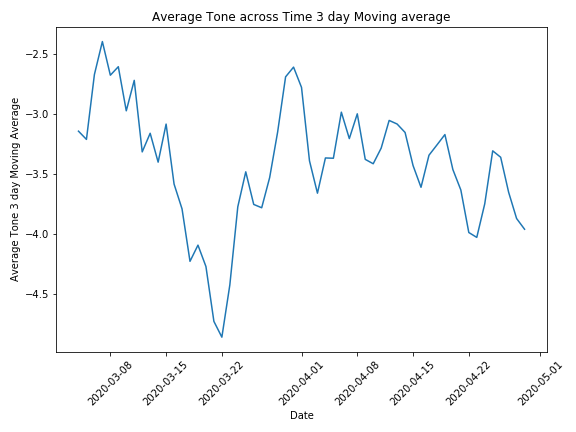
\includegraphics[width=0.49\textwidth]{images/avgtone_ma.png}\label{fig:avg_ma}}\\
 	\caption{GDELT Average Tone over time and Moving Average}
 	\label{fig:avg_tone_diff}
 \end{figure}
 
 Figure \ref{fig:gs_diff} shows the daily average of the Goldstein Scale of events across time, and as with the average tone plots, the 3 day moving average is shown in Figure \ref{fig:gs_ma}. The Goldstein Score, like the Average tone, appears to be chaotic, though in this case it shifts frequently from positive to negative. The moving average shows that there appears to be a peak halfway through the time period, followed by more fluctuation. 
 
 \begin{figure}[H]
 	\centering
 	\subfloat[GDELT Goldstein Scale]{  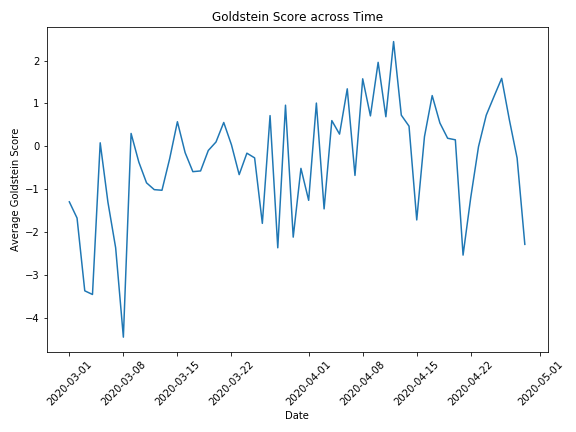
\includegraphics[width=0.49\textwidth]{images/goldsteinscore.png}\label{fig:gs}}
 	\subfloat[GDELT Goldstein Scale 3 Day Moving Average]{  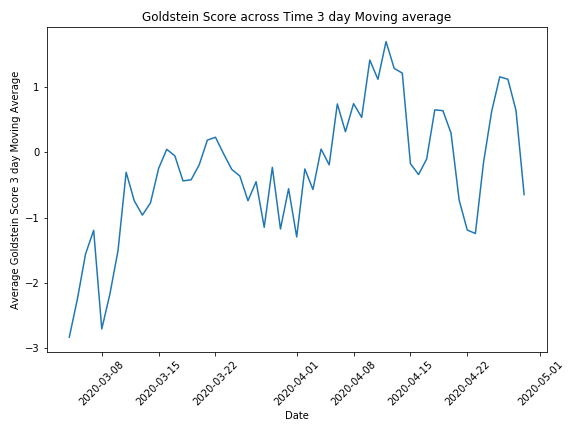
\includegraphics[width=0.49\textwidth]{images/goldsteinscore_ma.png}\label{fig:gs_ma}}\\
 	\caption{GDELT Goldstein Scale over time and Moving Average}
 	\label{fig:gs_diff}
 \end{figure}
 
 
\subsubsection{Stock Market Data}
Stock Market data was acquired from the yahoo! finance United Kingdom website. For the stock market data, the model would predict whether the stock would rise or fall over an entire day. Since there were potentially lots of events occurring on each day, the average was taken of the Goldstein scale and the Average Tone for all events on a specific day. 

Figure \ref{fig:dow_diff} shows the Dow difference between open and close prices on a daily basis. This data is fairly chaotic, with the difference jumping between positive and negative frequently and without an apparent pattern, thus a moving average of 3 days was plotted, which also remains slightly chaotic, but more trends appear. The market difference appears to be getting negatively larger towards the middle of the time period before recovering towards 0. The stock prices appeared to take a dive throughout March, which can be explained by the USA China trade flareups, and more pertinently, the impact of Covid-19.  The moving average also shows that the Dow Jones follows a slightly similar path with throughout time as the average tone, only a few days later, as the trough in the moving average for the Dow Jones difference occurs a few days after the trough in the average tone.

\begin{figure}[H]
	\centering
	\subfloat[Dow Jones Daily Difference]{  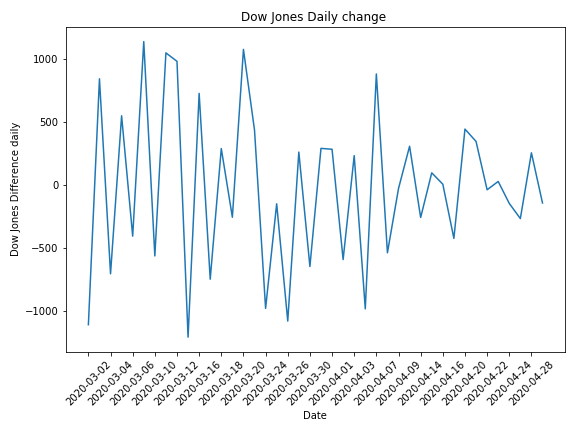
\includegraphics[width=0.49\textwidth]{images/dow_diff.png}\label{fig:diff}}
	\subfloat[Dow Jone Moving Average]{  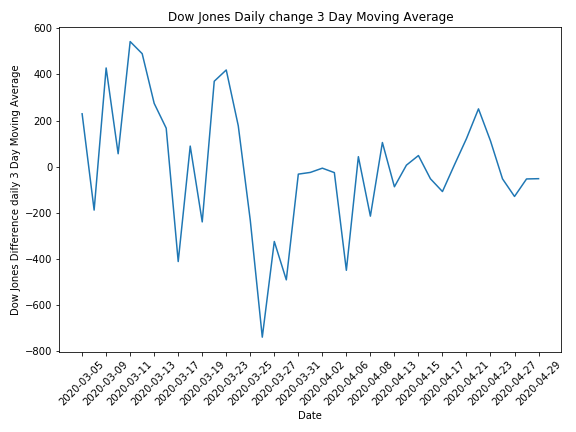
\includegraphics[width=0.49\textwidth]{images/dow_diff_ma.png}\label{fig:dow_diff_ma}}\\
	\caption{Dow Jones Daily Difference and Daily Difference Moving Average}
	\label{fig:dow_diff}
\end{figure}


\subsection{Topic Modelling}
There were several topic models run using several data sources. Firstly, a LDA model was run on a single day's GDELT event data. This was the whole day's worth of data with no country filter applied. This was to examine whether topic modelling was possible for the headlines data.  

The LDA models were applied on the USA/China GDELT data within the interval of the 1st of March to the 30th of April. 

After running the LDA models, the K means cluster models were run on the USA/China GDELT data with TF-IDF preprocessing.

\subsubsection{Preprocessing}
%The first topic model was fitted on one day data, using the gensim package. 
All of topic models worked on the basis of using a corpus for the data, This meant that the URLs were parsed, and then headlines taken from them. Each headline was used as a document, and split into the requisite words to be used. In this process the text was cleaned to remove punctuation and special characters, and formatted to build a corpus full of documents, with each document being a list of words from one URL. 
\subsubsection{TFIDF}
The TFIDF vectoriser present in the sklearn package was used to calculate the vector encodings, and was used as the basis of the cluster analysis for k means clustering. It was run across the USA/China filtered data to get an initial understanding of which terms would be most important across the dataset. This was then used to numerically transform the headlines for the K Means algorithm. 

\subsubsection{LDA}
To run the LDA model, the gensim package in the python programming language was used \cite{rehurek_lrec}. Several LDA models were fitted, each with a different number of topics, to examine which would be the best number of topics for the data. After the data was fitted, several phrases were inserted in the LDA model to see the probability of those words being in that topic or not. 

It was found that LDA models were only able to return a probability value for words which were already in the corpus. This meant that if there was a news headline related to the topics in the topic model but it contained a word not present in the corpus, it would mean that the topic model would not be able to say whether that news headline was part of that topic or not. This meant that this type of model could not be used to separate and filter irrelevant headlines from those headlines which were focused on the headlines in the model. 

\subsubsection{K Means}
K means clustering was also fitted on the data. The package used was the K Means clustering algorithm already implemented in the sklearn python package. Several cluster numbers were tried, from fitting with 2 centroids to fitting with 4 centroids. The Mahalanobis distance and the euclidean distance was calculated for each clusters' points. Furthermore, sample phrases were tested against k means models, to see if the cluster was meaningfully able to recognise the difference between words related to the clusters and noise in the algorithms. From an implementation perspective, a random seed was set for each of the clusters so the centres would start at the same point, and thus the results would be reproducible. 

To test the efficacy of the models with regards to filtering data, the Mahalanobis distance was calculated for each of the clusters for a selection of phrases. These phrases were varied in length and content. Some of the phrases were relevant to the main topics/content of the topic models, namely related to the pandemic, or the USA or China. Other phrases were completely unrelated to the topic models. If the cluster models were accurate in filtering information, the phrases closer to the topics at hand would be physically closer to the clusters in p-dimensional space and thus have smaller Mahalanobis distances than phrases which weren't close to the topics in hand.  

\subsection{Stock Modelling}
The main aim for this type of modelling was to predict whether the stock shifted up or down over the course of a day. Each day's difference was calculated between the opening and closing prices, and either a 1 or a 0 was used to represent the stock market going up and down. For the scope of the project, and similar to other modelling approaches, it was decided to only predict either the market going up or down. There were several models which were tried, detailed in \ref{models}. In all cases the response variable being predicted is the change in the stock price over a day. This takes a value of 1/0 for either a fall or rise. This is denoted Y at time t ($Y_{t}$), where t is a day, and ordered 1 to T, for the time interval used for training the model (April 1st to May 31st 2020). The predictors used were the Average Tone and Goldstein scale values for each day, along with differing amounts of predictors for previous day's data.

All of these models were tested and ranked on their accuracy. This was a percentage of the number of days that the model predicted whether the stock went up or down correctly. The `best` model was selected to be the one which had the highest accuracy values. The best model was then used to predict the stock shifts for the days between the 1st of May and the 30th of June, on the same set of data, i.e. the USA China GDELT filtered data. Another measure of the validity/accuracy of the best model was comparing it to a reference model. This reference model would use the same model type as the final model, but only use the previous day's stock shift, and \textit{not} the Average Tone or the Goldstein Scale values for predictions. 

\subsubsection{Preprocessing}
There was substantial preprocessing required for the data, first of all the stock market does not open on weekends or other holidays, however news and events do. Thus, the news over weekends was collated and averaged into the Friday figures. This meant that the prediction data had to the shifted, to ensure that information from the future was not being used to predict the data.

The next issue to consider whilst preprocessing the data was the issue of lag modelling. It is reasonable to expect that if there is an underlying relationship between the Goldstein Score/Average Tone and the stock price, a specific day's stock price changes would not restricted to just the previous day's news, but instead could be impacted by news over the previous several days. Thus the average scores and the Goldstein scales would have to be smoothed using several moving window calculations.

\subsection{Models}
\label{models}
All of the models tried were classification models, as by reducing the stock price changes into up or down, it became binary data. There were 4 main models which were tried, a Naive Bayes model, a Random Forests Model, a Support Vector Machine, and a simple Logistic Regression. Furthermore, a simple multi layer neural network was also tried on the data to see if there was any underlying representation that could be learned. All of the models were trained using 3 predictors, the Goldstein Score and the Average Tone of each day's events, and the previous day's stock change. 

Initially simple models were fitted with no moving average performed. However, it was assumed that an individual event could affect prices for several days, thus the Goldstein scale and Average tone predictors were smoothed using several different kinds of moving windows. There were 3 different moving window types tried, firstly a simple average was taken where each day was weighted evenly. The second method of moving window was an exponential decay window, and similarly a half Gaussian moving window. The moving windows were all spread over three days, as it was felt that this would provide the best balance at weighting past events evenly, without diluting the effect of the most recent news.

To test whether the previous N days' stock shift affected a specific day, three extra predictors were added, these predictors, along with the previous day's change, represented the stock shift for each of previous four days. These were used alongside the unsmoothed Average Tone and Goldstein Scale values to predict the stock prices. These models are henceforth referred to as the Manually Lagged Models.

All of these models were trained and tested on the March April data, and the results are reported in chapter \ref{results}.

To both show how this sort of predictive model would be used in the real world, and to test the `best` model's predictive capacity in `real` time, the `best` model was used to build a simple portfolio. For time reasons this only consisted of a single stock, where shares were bought or sold on a daily basis based on the model's confidence in the following day's stock shift. This was to mimic the behaviour of being used in real time, where there would only be new news for the current day, and based on the previous news and each day's news, the next day's prediction would be made. The stock chosen was Apple Inc. as this stock had the highest weighting in the Dow Jones index. The Apple historical data values were also procured from the finance Yahoo United Kingdom website. 

This was a very simple portfolio test, where each day's prediction triggered buying and selling of the stocks, i.e. stock was only ever held when the confidence of market shift was not above a threshold, otherwise stock would be bought and sold daily. There were several hyperparameters involved, namely these were the initial capital, initial number of shares, the confidence threshold required to trigger buying or selling stocks. There were also two additional hyperparameters, these variables controlled the fraction of capital used to buy stock, or the buy-factor, and the fraction of stock to sell at any given point, sell-factor. These variables were constant for every run, so for one test on the May to June, every time the confidence in the prediction for the next day was greater than the confidence threshold, and the market was predicted to increase, the buy-factor amount of the capital at that point was used to `purchase` stock. The reverse happened when the market was projected to decrease, with the sell-factor fraction of the stock being held being sold. Since geopolitical events can occur after the market close which are factored in by the predictive model, the stock close price was used as the reference price for buying and selling stock. 

For the May to June time period, the number of shares, and the capital was tracked, along with the total asset value, which was the total capital plus the monetary value of those shares at the closing price each day.

The `best` predictive model's portfolio was also compared to a portfolio which used the reference model, and the results are shown in chapter \ref{results}.
